\documentclass{article}
  %----------------------------------------------------------------------------------------
%	Author:	WangYifu
%	Create Date:	2017-02-14
%	Last Modify:	2018-09-01
%----------------------------------------------------------------------------------------
\usepackage[T1]{fontenc}
\usepackage{fourier}
\usepackage[english]{babel}
\usepackage{amsmath,amsfonts,amsthm}
\usepackage{geometry}
\usepackage{fancyhdr}
\usepackage{listings}
\usepackage{color}
\usepackage[yyyymmdd]{datetime}
\usepackage{graphicx}
\usepackage{float}
\usepackage{titling}
\usepackage{titlesec}
%-------------------------------%
%          Page Style           %
%-------------------------------%
\pagestyle{fancyplain}
\fancyhead{}
\fancyfoot[L]{}
\fancyfoot[C]{}
\fancyfoot[R]{\thepage}
\renewcommand{\headrulewidth}{0pt}
\renewcommand{\footrulewidth}{0pt}
\setlength{\headheight}{13.6pt}
\textwidth=6.5in
\textheight=9.0in
\headsep = 0.1in
\renewcommand{\baselinestretch}{1.2}
\geometry{a4paper,left=2cm,right=2cm,top=2cm,bottom=2cm}

%-------------------------------%
%           Font Size           %
%-------------------------------%
\newcommand{\erhao}{\fontsize{22.1pt}{\baselineskip}\selectfont}
\newcommand{\sanhao}{\fontsize{16.1pt}{\baselineskip}\selectfont}
\newcommand{\sihao}{\fontsize{14.1pt}{\baselineskip}\selectfont}
\newcommand{\xiaosi}{\fontsize{12.1pt}{\baselineskip}\selectfont}
\newcommand{\wuhao}{\fontsize{10.5pt}{\baselineskip}\selectfont}
\newcommand{\setFontSize}[1]{\fontsize{#1}{\baselineskip}\selectfont}
\titleformat{\section}{\sanhao\bfseries}{$\bullet$}{5pt}{}

%-------------------------------%
%             Title             %
%-------------------------------%
\newcommand{\horrule}[1]{\rule{\linewidth}{#1}}
\renewcommand{\dateseparator}{ - }
\def\Assignment{Assignment Title}
\title{
\vspace{-2cm}
\normalfont \normalsize
\textsc{Washington University in St. Louis} \\ [0pt]
\horrule{1pt} \\[0.4cm]
\huge {\bf\Assignment}
}
\author{467261 - Yifu Wang}
\date{\normalsize\today\\\horrule{1pt} \\[0.5cm]}

%-------------------------------%
%           TableList           %
%-------------------------------%
\newcommand{\deflabel}[1]{#1\hfill}
\newenvironment{tlist}[1]{
	\begin{list}{}{
			\settowidth{\labelwidth}{\bf#1}
			\setlength{\leftmargin}{\labelwidth}
			\addtolength{\leftmargin}{\labelsep}
			\renewcommand{\makelabel}{\bf\deflabel}}}{
	\end{list}
}

%-------------------------------%
%             Code              %
%-------------------------------%
\definecolor{gray}{RGB}{191,191,191}
\definecolor{dkgreen}{RGB}{96,139,78}
\definecolor{mauve}{RGB}{206,145,120}

\lstset{ %
	language=C++,                % the language of the code
	% basicstyle=\textheight,           % the size of the fonts that are used for the code
	numbers=left,                   % where to put the line-numbers
	numberstyle=\color{black},  % the style that is used for the line-numbers
	stepnumber=0,                   % the step between two line-numbers. If it's 1, each line 
	% will be numbered
	numbersep=5pt,                  % how far the line-numbers are from the code
	backgroundcolor=\color{gray},      % choose the background color. You must add \usepackage{color}
	showspaces=false,               % show spaces adding particular underscores
	showstringspaces=false,         % underline spaces within strings
	showtabs=false,                 % show tabs within strings adding particular underscores
	frame=false,                   % adds a frame around the code
	rulecolor=\color{gray},        % if not set, the frame-color may be changed on line-breaks within not-black text (e.g. commens (green here))
	tabsize=2,                      % sets default tabsize to 2 spaces
	captionpos=b,                   % sets the caption-position to bottom
	breaklines=true,                % sets automatic line breaking
	breakatwhitespace=false,        % sets if automatic breaks should only happen at whitespace
	keywordstyle=\color{blue},          % keyword style
	commentstyle=\color{dkgreen},       % comment style
	stringstyle=\color{mauve},         % string literal style
}

  \def\Assignment{CES571S - L2 - Crypto Encryption}
\begin{document}
\maketitle
\section{Substitution Cipher}
I didn't reinvent the crypto algorithm for substitution cipher. I did some research in this field and use the substitution solver to solve this online. The following steps is the path I will take to implement a solver by myself.
\begin{tlist}{3}
	\item[1.]
	Scan the ciphertext, record the frequency of each letter, record the frequency of each 1-letter, 2-letter, 3-letter words, record the pattern of two consequent same letter.
	\item[2.]
	The frequency of what we recorded in step one in plaintext of English should be
	\begin{tlist}{0}
		\item[letter:]\{ETAOIN/RSHDL\}>0.04, \{CU/FMPGWY\}>0.02, \{BV/KXJQZ\}<0.02
		\item[1-letter word:]a, i
		\item[2-letter word:]of, to, in, it, is, be, as, at, so, we, he, by, or, on, no...
		\item[3-letter word:]the, and...
		\item[consequent pattern:]ss, ee, tt, ff, ll, mm, oo...
	\end{tlist}
	\item[3.]
	Sort the a-z letters by the frequency we recorded and use this as an initial key for our algorithm. This algorithm could be Hill Climbing, Simulated Annealing or Genetic Algorithm. In order to find the best solution which make our translated text fit the frequency table listed in step 2 best. We need a algorithm to measure the fitness of current solution. This algorithm can be as simple as measure how close a 'out-of-order' sequence to a 'well-ordered' sequence.
	\item[4.]
	After we get the solution from step 3. The key we obtained might be still not right. Then we exchange the letter in the same group in the \textbf{letter} listed in step 2 by exhaustive method. Quit the algorithm once the grading of current solution exceed the pre-set threshold.
\end{tlist}
Here is the \href{http://freetexthost.com/j54kutb05a}{solution} I obtained and the \href{https://www.guballa.de/substitution-solver}{solver} I used.

\section{Encryption Mode - ECB vs. CBC}
This task is somehow related to another course I take, CSE554T, where we learn to process 2D or 3D img data using Mathematica language. It's a interactive programming language. I choose use it for this task and I upload the source code to \href{https://github.com/Luna1996/WUSTL/blob/master/571/L2/task2.m}{github}. The following is a simple explaination of the code.
\begin{tlist}{3}
	\item[1.]\code{KeyGen} generate a L-byte-long random key.
	\item[2.]The block cipher used in \code{ECB} and \code{CBC} are \code{BitXor} for simple.
	\item[3.]The IV used in \code{CBC} is randomly generated, since we didn't really need to decrypt the image.
\end{tlist}
The following 3 images are origin, ECB and CBC.
\begin{figure}[H]\centering
\includegraphics{pic_original.png}\end{figure}
\begin{figure}[H]\centering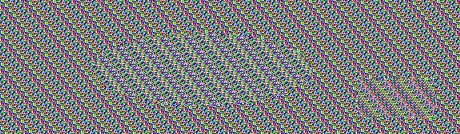
\includegraphics{pic_ecb.png}\end{figure}
\begin{figure}[H]\centering
\includegraphics{pic_cbc.png}\end{figure}
You can see that the encrypted img produced by ECB still preserve the shape of original img. That is because when using an ECB same plaintext will be encrypted into same ciphertext. By applying CBC you can eliminate such disadvantage.\\
Following 3 images reproduce this phenomenon using another original image.
\href{https://i.loli.net/2018/09/24/5ba874d18c3b5.jpg}{original}
\href{https://i.loli.net/2018/09/24/5ba874d19386e.jpg}{ECB}
\href{https://i.loli.net/2018/09/24/5ba874d193869.jpg}{CBC}

\section{Error Propagation - Corrupted Cipher Text}
To answer the question first.
\begin{tlist}{2}
	\item[$\bullet$]\textbf{ECB,OFB} will only affect the block where the corruption happend.
	\item[$\bullet$]\textbf{CBC,CFB} will affect the block where the corruption happend and the block after it.
\end{tlist}
In order to observe the corruption easily. The plaintext I choose will be character \code{'1'} repeated 1008 times.
I used Javascript with the package 'aes-js' to perform this task. I encountered several truble by doing so.
\begin{tlist}{2}
	\item[$\bullet$]I have tried another famouse npm package for crypto, 'crypto-js', but I couldn't corrupt the ciphertext produced by it. It seems that 'crypto-js' do extra work to make sure ciphertext is untouched.
\end{tlist}
Here is the \href{https://github.com/Luna1996/WUSTL/blob/master/571/L2/task3.js}{source code}. And the results: (the block refers to the block locate at corrupt point)
\begin{tlist}{2}
	\item[$\bullet$]
	\href{https://github.com/Luna1996/WUSTL/blob/master/571/L2/ecb.txt}{\textbf{ECB}}
	only the block breaks.
	\item[$\bullet$]
	\href{https://github.com/Luna1996/WUSTL/blob/master/571/L2/cbc.txt}{\textbf{CBC}}
	and
	\href{https://github.com/Luna1996/WUSTL/blob/master/571/L2/cfb.txt}{\textbf{CFB}}
	only the block and the block after it.
	\item[$\bullet$]
	\href{https://github.com/Luna1996/WUSTL/blob/master/571/L2/ofb.txt}{\textbf{OFB}}
	every block break, totally unreadable.
\end{tlist}
The result of OFB is unexpected. Which I don't understand. From the definition in \href{https://i.loli.net/2018/09/24/5ba8a461a5228.png}{this picture}. And from the mathematical definition
$$
	\begin{aligned}
		C_i & =\ P_i\oplus O_i \\
		P_i & =\ C_i\oplus O_i \\
		O_i & =\ E_k(O_{i-1})  \\
		O_0 & =\ IV
	\end{aligned}
$$
It seems that the single byte corruption won't cause any propagation.

\section{Initial Vector}
\subsection{}
The Javascript source code is upload to
\href{https://github.com/Luna1996/WUSTL/blob/master/571/L2/task41.js}{github}.
The plaintext is
\begin{center}
	\code{'The quick brown fox jumps over the laze dog.\ \ \ \ '}
\end{center}
\code{key}, \code{iv1} and \code{iv2} are randomly generated. \code{e1} and \code{e2} using \code{iv1} as IV, \code{e3} using \code{iv2}. \code{e1} and \code{e2} are excatly same. Here is the \href{https://i.loli.net/2018/09/25/5ba9b6889cf97.png}{screen shot}. Thus since using same IV will cause the same plaintext encrypted into the same ciphertext. It's vulnerable under strong attacking.
\subsection{}
Yes we can. Since we have
$$
	\begin{aligned}
		C_i & =\ P_i\oplus O_i \\
		P_i & =\ C_i\oplus O_i \\
		O_i & =\ E_k(O_{i-1})  \\
		O_0 & =\ IV
	\end{aligned}
$$
thus $O_i = C_i\oplus P_i$. Furthermore if IV remains same, all $O_i$ will remain same. By running \href{https://github.com/Luna1996/WUSTL/blob/master/571/L2/task42.js}{this algorithm}. We have
\begin{center}
	\code{P2 = 'Order: Lauch a missile!'}
\end{center}
If we replace OFB with CFB. We will at least reveal the first bolck of \code{P2}. Since by the definition
$$
	\begin{aligned}
		C_i & =\ E_K(C_{i-1})\oplus P_i \\
		P_i & =\ E_K(C_{i-1})\oplus C_i \\
		C_0 & =\ IV
	\end{aligned}
$$
only $C_0$ will remain unchanged between two cipher processes.
\subsection{}
The definition of CBC is (only one block)
$$
	\begin{aligned}
		C1 & =\ E_K(IV1\oplus P1) \\
		C2 & =\ E_K(IV2\oplus P2)
	\end{aligned}
$$
Thus if we construct
$$P2 = IV2 \oplus IV1 \oplus P1$$
we shall get $C1 = C2$. The Javascript source code is uploaded to github. And from the debug view, we can see \code{P1 = Yes}.\\
When conduct this attacking. I encountered a truble. That is when the plaintext is not a multiple of 16 (key size in byte). aes-js package will throw a error and refuse to continue any calculation. And I don't know what has been append to the P1 by default. So I have to using the key (known only to Bob) to decrypt the C1 and found out that \code{'\r'}s have been added to make a 16 length P1. And the code of \code{'\r'} is 13. That's the reason of line 11.

\end{document}